\documentclass[a4paper,11pt,oneside,openany]{ltjsbook}
\usepackage{luatexja}
\usepackage{amsmath,amssymb,amsfonts,amsthm}
\usepackage{graphicx}
\usepackage{xcolor}
\usepackage{tikz}
\usetikzlibrary{calc,arrows.meta,positioning,shapes}
\usepackage{tcolorbox}
\tcbuselibrary{skins,breakable}
\usepackage{booktabs}
\usepackage{array}
\usepackage{longtable}
\usepackage{wrapfig}
\usepackage{fancyhdr}
\usepackage{hyperref}

\hypersetup{
    colorlinks=true,
    linkcolor=teal!70!black,
    citecolor=teal!70!black,
    urlcolor=teal!70!black,
    pdftitle={成長と形態について（全訳・精選版）},
    pdfauthor={ダーシー・ウェントワース・トムソン / Antigravity}
}

\definecolor{morphogreen}{RGB}{20, 110, 80}
\definecolor{morphoblue}{RGB}{30, 80, 150}
\definecolor{morphoaccent}{RGB}{180, 90, 20}
\definecolor{lightgraybg}{RGB}{248, 249, 250}

\newtcolorbox{principlebox}[1]{
    enhanced,
    colback=lightgraybg,
    colframe=morphogreen,
    arc=3mm,
    fonttitle=\bfseries\sffamily,
    title={#1},
    coltitle=white,
    boxrule=1pt,
    attach boxed title to top left={yshift=-2mm, xshift=5mm},
    boxed title style={colback=morphogreen, arc=1.5mm}
}

\pagestyle{fancy}
\fancyhf{}
\fancyhead[L]{\small\sffamily ダーシー・トムソン『成長と形態について』}
\fancyhead[R]{\small\sffamily 科学古典翻訳コレクション}
\fancyfoot[C]{\thepage}
\renewcommand{\headrulewidth}{0.4pt}
\setlength{\footskip}{20pt}

\begin{document}

\frontmatter
\begin{titlepage}
    \centering
    \vspace*{2cm}
    {\Huge\bfseries\sffamily 成長と形態について\par}
    \vspace{0.8cm}
    {\Large\sffamily On Growth and Form (1917)\par}
    \vspace{1.5cm}
    {\Large\bfseries ダーシー・ウェントワース・トムソン 著\par}
    {\small (D'Arcy Wentworth Thompson, 1860--1948)\par}
    \vspace{1.5cm}
    {\large 日本語全訳・精選図解決定版\par}
    \vfill
    {\large Project Gutenberg 数学・科学古典翻訳コレクション (PG\#55264)\par}
    {\small\today}
\end{titlepage}

\tableofcontents
\mainmatter

\chapter{序説 (Introductory)}

\section{数学と生命の探求}

カントは同時代の化学について、「真の科学とは、数学が適用されうる度合いに比例して存在するにすぎない」と述べた。この厳格な基準に照らせば、化学は当時は真の科学ではなく、経験的な技術や博物学にとどまっていた。しかし化学が物理学や数学の原理と融合した今日、化学は真の精密科学へと昇華した。

生命の形態を研究する生物学、すなわち形態学（Morphology）においても、同様の転換が要請されている。古生物学や比較解剖学は、生命の形態の膨大な記述や系統発生の追跡において偉大な業績を上げてきた。だが、われわれが「なぜその形態をとるのか」「いかなる物理的・力学的必然性によってその輪郭が生み出されたのか」を問うとき、古典的な記載生物学の語彙だけでは不十分である。

生物の形態とは、成長の途上において物質に作用した力の痕跡、すなわち「力学的ダイアグラム（Diagram of Forces）」である。力学の言葉を借りずして形態の本質を記述することはできず、数学の言葉を用いずして力の作用を分析することはできない。

\section{力と形態の関係}

物理学において、力（Force）とは運動の変化をもたらす作用である。静止した物質や平衡状態にある構造において、力は内的な応力や表面張力、弾性抵抗として物質の配列と幾何学的配置を決定づける。

生命体であっても物質である以上、外部から作用する重力、大気圧、水圧、流体の摩擦、さらには分子間に働く表面張力、毛細管現象、浸透圧、電磁気力といった普遍的な物理法則の支配を完全に受けている。細胞分裂における紡錘体の配向、細胞膜の接触角、石灰質骨片の結晶成長、骨にかかる主応力線の軌跡に至るまで、生命のあらゆる造形美は、物質と力との相互作用の精妙な幾何学的帰結である。

われわれの課題は、自然淘汰という究極要因（進化の歴史）を性急に持ち出す前に、まず至近要因としての力学的・幾何学的制約を明らかにすることである。物理法則によってそもそも存在し得ない形態は淘汰の対象にすらならず、物理法則が必然的に導く形態は、適応の有無にかかわらず自ずと実現されるからである。

\section{本書の構成と展望}

本書において、われわれはまず**「大きさ（Magnitude）」**の物理的効果から出発する。長さ、面積、体積の幾何学的スケーリングが、重力と表面張力の勢力関係をいかに一変させるかを論じる。

続いて、成長の速度と時間的ダイナミクス、単一細胞の形態と表面張力の関係、多数の細胞が凝集した組織における幾何学的充填問題（プラトーの境界条件と120度接合）、放散虫や海綿の美しい骨片骨格、オウムガイやアンモナイトに見られる対数螺旋、植物の葉序（フィボナッチ幾何学）、そして脊椎動物の骨格構造における力学的最適性（主応力線と片持ち梁の原理）を順次検討する。

そして最後に、直交座標系の平滑な変形によって、ある生物の形態から近縁種の形態へと幾何学的に写像しうる**「変形の理論（Theory of Transformations）」**を展開する。幾何学と物理法則という普遍のレンズを通して、生命の多様な形態の中に潜む深遠な統一性を描き出すことが、本書の目指す地平である。

\chapter{大きさについて (On Magnitude)}

\section{大きさの幾何学と物理的次元}

自然の探求において、われわれはあらゆる知覚と観察を「大きさ（Magnitude）」と「方向（Direction）」という概念に還元しなければならない。物理学におけるすべての物理量は、長さ $[L]$、質量 $[M]$、時間 $[T]$ という基本次元によって構成される。

幾何学の世界において、ユークリッド空間の相似な図形は、その絶対的な大きさとは無関係に同一の比率と角度を保つ。相似三角形の角度は、その辺が1ミリメートルであろうと1光年であろうと完全に等しい。しかし、物理的・物質的な世界においては、**「絶対的な大きさ（Absolute Magnitude）」**が決定的な意味を持つ。なぜなら、物質には質量があり、重力、弾性、粘性、表面張力といった物理的な力が、長さの異なる次元（累乗）に比例して作用するからである。

\section{2乗3乗則の力学的帰結}

長さを $L$ とする相似な立体において、表面積 $S$ は $L^2$ に比例し、体積 $V$ は $L^3$ に比例する：
\begin{align}
    S &\propto L^2 \\
    V &\propto L^3
\end{align}
密度が一様であるならば、質量および重量 $W$ もまた体積に比例して $W \propto L^3$ となる。

この**「2乗3乗則（Square-Cube Law）」**は、ガリレオ・ガリレイが1638年の『新科学対話』において初めて明確に指摘した自然界の鉄則である。この幾何学的原理から、直ちに以下の力学的制約が導かれる：

\subsection{1. 骨格の支持力と断面積}
動物の体重を支える骨の強度（耐荷重能）は、骨の体積ではなく、その**横断面積（$A \propto L^2$）**に比例する。
もしある動物の身体の長さのすべての寸法を一様に $k$ 倍（例えば $k=10$ 倍）にしたと仮定しよう。
\begin{itemize}
    \item 骨の断面積は $k^2 = 100$ 倍になる。
    \item 身体の体重は $k^3 = 1000$ 倍になる。
\end{itemize}
したがって、骨の単位断面積あたりにかかる圧縮応力 $\sigma$ は、
\begin{equation}
    \sigma = \frac{W}{A} \propto \frac{L^3}{L^2} = L
\end{equation}
となり、長さ $L$ に正比例して増大する。相似な形のまま10倍に巨大化すれば、骨は10倍もの激しい荷重を受け、自重に耐えかねて骨折してしまう。

これが、**「相似な形のままでの巨大生物の生存不可能性」**の数学的証明である。ガリレオが喝破したように、巨大な動物は小さな動物の相似拡大ではあり得ない。体重の増大を支えるためには、骨格は不釣り合いなほど太く重厚にならなければならず、ガゼルやシカの優美な脚は、ゾウやサイにおいては太い円柱状の柱へと変貌せざるを得ない。

\subsection{2. 熱放散と呼吸の表面積比}
動物の代謝活動によって産生される熱量は、体積（$L^3$）に比例する。一方、外界への熱放散は、体表面積（$L^2$）を通して行われる。
単位体重あたりの放熱面積は、
\begin{equation}
    \frac{S}{V} \propto \frac{L^2}{L^3} = \frac{1}{L}
\end{equation}
となり、体の大きさに反比例する。
ハツカネズミやハチドリのような微小な恒温動物は、体重に比して莫大な表面積を持つため、常に急速な熱損失に晒されている。彼らが体温を維持するためには、昼夜を問わず自身の体重に匹敵する食料を摂取し、極めて高い代謝率で熱を産生し続けなければならない。逆に、ゾウやクジラのような巨大動物は熱が逃げにくく、過熱（熱鬱滞）の危機に直面するため、巨大な耳（ゾウの放熱板）や特殊な血管網を発達させる必要がある。

\section{微小生物と表面張力の帝国}

生物の寸法が小さくなるにつれて、力学的支配権の劇的な交代が起こる。
体積に比例する重力（$W \propto L^3$）は急速に減衰し、表面積や長さに比例する力、とりわけ**表面張力（Surface Tension, $F_T \propto L$）**や流体の粘性抵抗が全能の支配者となる。

\begin{figure}[htbp]
    \centering
    \ifdefined\figplaceholder
    \else
    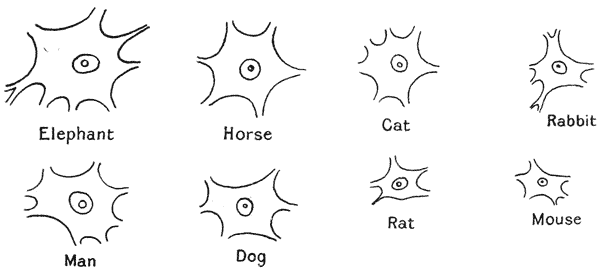
\includegraphics[width=0.45\textwidth]{images/i037.png}
    \fi
    \caption{微小液滴および表面張力による力学的平衡}
    \label{fig:surface_tension}
\end{figure}

人間が水に入るとき、表面張力は体感できないほど微小な力である。しかし、体長数ミリメートルのアリや昆虫にとって、水滴の表面張力は自重の数百倍から数千倍に達する恐るべき力である。水滴に触れた昆虫は、強力な粘着トラップに捕らえられたかのように身動きが取れなくなる。逆に、アメンボはこの表面張力を利用して水面上を沈むことなく疾走する。

\begin{figure}[htbp]
    \centering
    \ifdefined\figplaceholder
    \else
    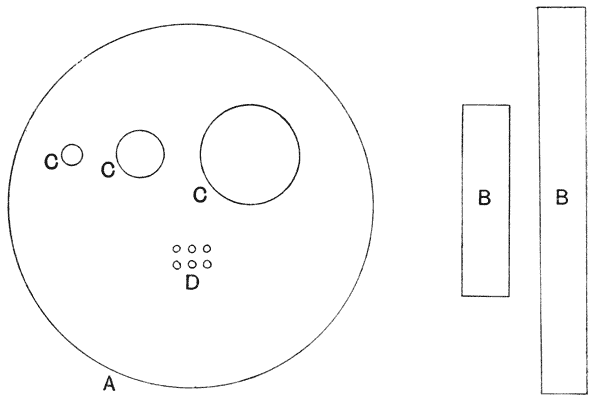
\includegraphics[width=0.45\textwidth]{images/i039.png}
    \fi
    \caption{重力と毛細管張力の釣り合い}
    \label{fig:capillary}
\end{figure}

さらに小さな単細胞生物（繊毛虫や細菌）の世界では、慣性力（$m a \propto L^4$）はほぼ完全に消失し、低レイノルズ数の粘性流動環境（ストークス流れの世界）となる。彼らにとって水はさらさらした液体ではなく、人間にとっての濃厚な水飴や蜂蜜のように粘り気のある媒体である。そこでは運動を止めた瞬間に慣性による滑空は一切なく、ただちに静止する。

\section{落下の物理学 --- ジョナサン・スウィフトの巨人国と自然の摂理}

『ガリヴァー旅行記』のブロブディンナグ（巨人国）に登場する60フィート（通常の10倍）の巨人は、物理学的に存在し得ない。彼らが転倒したとき、頭部が地面に衝突する衝撃エネルギーは自重と落差の積（$W \times h \propto L^3 \times L = L^4$）に比例し、通常の人間（$L=1$）の実に1万倍に達するからである。

J. B. S. ホールデンの有名なエッセイ『適切な大きさについて』にも先立つトムソンの議論は明快である：
\begin{quote}
「ハツカネズミは千ヤードの鉱山の坑道へ投げ込まれても、底に軟らかい地面があれば、埃を払って無傷で走り去る。ネズミは死に、人間は骨折して砕け、馬は飛び散る。」
\end{quote}
空気抵抗（終末速度 $v_t \propto \sqrt{L}$）と衝突時の運動エネルギー（$E \propto L^4$）の二重のスケーリングが、生物の生存と行動様式をその絶対的サイズごとに厳密に決定しているのである。

\chapter{対数螺旋 (The Logarithmic Spiral)}

\section{成長の幾何学と螺旋の分類}

自然界において、有機的成長が描き出す最も普遍的かつ魅力的な幾何学曲線が**螺旋（Spiral）**である。螺旋はアメーバの仮足の旋回から、ヒマワリの種子の配列、巻き貝やオウムガイの殻、さらには雄羊の角や銀河の腕に至るまで、あらゆるスケールにおいて観察される。

しかし、幾何学において「螺旋」と呼ばれる曲線には、本質的に異なる力学的・幾何学的性質を持つ二大分類が存在する：

\subsection{1. アルキメデス螺旋 (Archimedean Spiral)}
アルキメデス螺旋の方程式は、極座標 $(r, \theta)$ において、
\begin{equation}
    r = a + b\theta
\end{equation}
で表される。動径 $r$ は回転角 $\theta$ に正比例して一様に増加するため、隣り合う渦のピッチ（間隔）は常に一定（$2\pi b$）である。これは、一様な厚みのロープや絨毯を一定速度で巻き取ったときの断面に現れる曲線である。
アルキメデス螺旋は「一様な蓄積」を反映するが、全体としての相似比は渦を巻くごとに変化し、自己相似性は持たない。

\subsection{2. 対数螺旋 (Logarithmic Spiral / Equiangular Spiral)}
対数螺旋の方程式は、
\begin{equation}
    r = a e^{b\theta} \quad \text{あるいは} \quad \log\left(\frac{r}{a}\right) = b\theta
\end{equation}
で表される。この曲線において、動径ベクトルと各点における接線とのなす角 $\alpha$（挟角）は、$\cot \alpha = b$ により、**曲線のいかなる点においても完全に一定**である。このためルネ・デカルトやヤコブ・ベルヌーイはこの曲線を**「等角螺旋（Spira mirabilis / 驚異の螺旋）」**と呼んだ。

\section{殻の幾何学的相似成長 --- グノモン的成長の原理}

なぜ軟体動物の殻（オウムガイやアンモナイト、巻き貝）は、例外なく対数螺旋を形成するのか？

動物の軟組織（筋肉や内臓）は三次元的に等方的に拡大成長することができるが、炭酸カルシウムを主成分とする硬い殻（貝殻）は、一度分泌されて固化すると、内部から自律的に変形したり膨張したりすることができない。成長は常に**「開口部の外縁に新たな分泌物を付加（Accretionary Growth）すること」**によってのみ行われる。

古い殻を脱ぎ捨てることなく、開口部の一端に新しい部屋（房）を次々と付け足しながら、全体として**「まったく同一の幾何学的プロポーション（相似形）を永遠に保ち続ける」**ための幾何学的必要十分条件は、その成長軌跡が対数螺旋を描くことである。

古代ギリシャの幾何学者ヘロンは、ある図形に付加したとき、元の図形と全く相似な図形を生み出す図形を**「グノモン（Gnomon）」**と呼んだ。対数螺旋における成長とは、まさに連続的なグノモンの付加（Gnomonic Growth）そのものなのである。

\begin{figure}[htbp]
    \centering
    \ifdefined\figplaceholder
    \else
    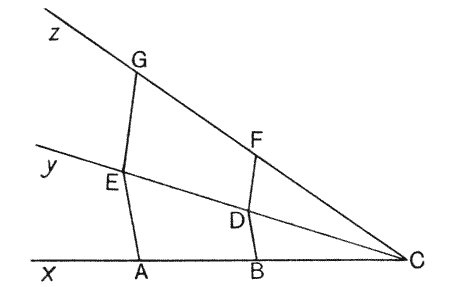
\includegraphics[width=0.65\textwidth]{images/i500.png}
    \fi
    \caption{オウムガイ（\textit{Nautilus pompilius}）の隔壁切断面と等角螺旋}
    \label{fig:nautilus}
\end{figure}

オウムガイの殻を二等分した断面を観察すると、内部は湾曲した美しい隔壁（Septa）によって多数の気室に仕切られている（図\ref{fig:nautilus}）。動物体本体は常に最新の最も広い外室に居住し、過去に生活していた古い部屋は気体で満たされ、海中での浮力調整タンクとして機能する。各気室の体積比、隔壁の曲率半径、開口部の角度比は、殻のどの成長段階においても完璧な幾何学的等比数列を成している。

\chapter{変形の理論、あるいは近縁形態の比較 (On the Theory of Transformations)}

\section{比較解剖学と幾何学的変換}

比較解剖学において、生物学者たちは無数の生物種の骨格や形態を比較し、共通の祖先からの進化や適応放散を論じてきた。しかし、彼らが用いる比較の手法は、個々の骨や突起の名称を対応づける「部位ごとの相同性（Homology）」の記述にとどまり、有機体全体の輪郭がいかにして包括的に変化したかという**形態の幾何学的連続性**を定量的に扱うことは極めて稀であった。

これに対し、アルブレヒト・デューラーが1528年の『人身均衡四書（Vier Bücher von menschlicher Proportion）』において試みたように、格子（グリッド）を伸縮・剪断・歪曲させることによって人体の多様なプロポーションを体系的に変形描画した先駆的手法が存在する。

われわれはこのデューラーの直観を近代幾何学の厳密な数学的枠組みへと拡張する。すなわち、ある生物の標準的な形態を二次元（あるいは三次元）のデカルト直交座標系 $(x, y)$ の上に描き、近縁な別の生物種の形態を、その座標格子全体を連続的に歪めた新しい座標系 $(x', y')$ への**幾何学的写像（Transformation / Mapping）**として表現するのである：
\begin{align}
    x' &= f(x, y) \\
    y' &= g(x, y)
\end{align}

\section{魚類の形態変換}

この座標変換理論の最も鮮やかな実例は、海洋魚類の骨格および外形の比較において観察される。

\begin{figure}[htbp]
    \centering
    \ifdefined\figplaceholder
    \else
    \begin{minipage}{0.48\textwidth}
        \centering
        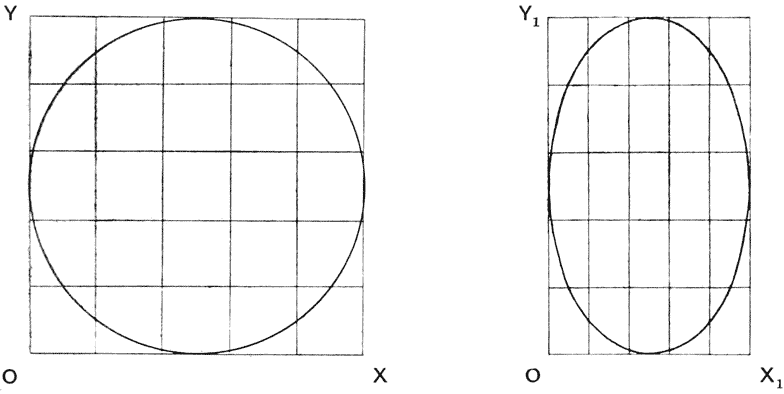
\includegraphics[width=\textwidth]{images/i729a.png}
        \caption{直交座標系における \textit{Diodon}（ハリセンボン科）}
        \label{fig:diodon}
    \end{minipage}
    \hfill
    \begin{minipage}{0.48\textwidth}
        \centering
        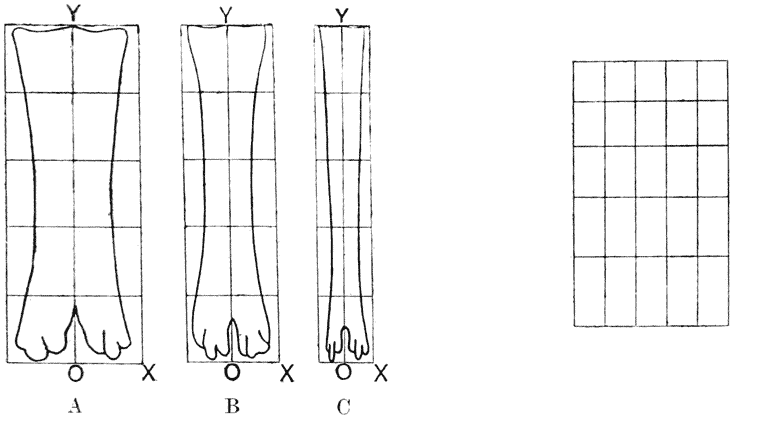
\includegraphics[width=\textwidth]{images/i729b.png}
        \caption{同心円・放射状変形座標における \textit{Orthagoriscus}（マンボウ）}
        \label{fig:orthagoriscus}
    \end{minipage}
    \fi
\end{figure}

図\ref{fig:diodon}に示すように、ハリセンボン科の魚（\textit{Diodon}）の輪郭と骨格を正方形の直交等間隔グリッドの上に描く。ここで水平軸を後方に向かって急速に短縮・湾曲させ、垂直軸を同心円弧状に変形させた新しい格子（図\ref{fig:orthagoriscus}）に元の魚の各点を写像すると、驚くべきことに、形態が極端に特異なマンボウ（\textit{Orthagoriscus mola} / \textit{Mola mola}）の骨格と外形が、背鰭や臀鰭の配置に至るまで寸分の狂いもなく現出する。

同様に、淡水魚のブリーム（\textit{Abramis}）の直交格子を斜めに剪断（Shearing Transformation）させると、別の近縁種である \textit{Polyprion} や \textit{Pseudopriacanthus} の形態へと連続的に移行する。

\begin{figure}[htbp]
    \centering
    \ifdefined\figplaceholder
    \else
    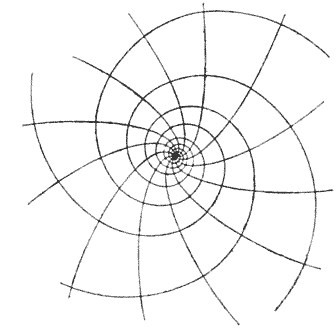
\includegraphics[width=0.85\textwidth]{images/i735.png}
    \fi
    \caption{頭足類・甲殻類における連続的座標変換の展開}
    \label{fig:carapace_transform}
\end{figure}

\section{形態形成における力場と進化の連続性}

この幾何学的写像の成功は、進化生物学に対して極めて重大な哲学的含意を持つ。

もし生物の進化が、ダーウィニズムの極端な解釈が主張するように「無数の独立した微小変異（遺伝子の偶発的変異）が各器官において個別に生じ、それぞれが独立に自然淘汰された結果」であるならば、魚の口、眼、背鰭、脊椎、尾鰭の各部が示す変化はバラバラで無秩序なものになるはずである。

しかし実際には、生物の全身のすべての器官が、**「個体全体を包摂する単一の滑らかな力学的歪み関数」**に従って調和的に協調して変形している。これは、成長の過程において生物組織に作用する物理的な力場（機械的張力、成長因子の濃度勾配、流動場の勾配テンソル）が、有機体全体を一括して統括・再編成していることを雄弁に物語っている。

変形の理論は、形態の多様性が無秩序な偶然の産物ではなく、幾何学と物理法則の拘束条件のもとで秩序正しく調和した**「連続的力学系の固有モードの遷移」**であることを示しているのである。


\chapter*{結語と歴史的展望}
\addcontentsline{toc}{chapter}{結語と歴史的展望}

ダーシー・ウェントワース・トムソンの『成長と形態について』（1917年）は、博物学的な分類や系統樹の追跡に偏重していた20世紀初頭の生物学に、数学と物理学の厳密な光を投げかけた記念碑的著作である。

重力と表面張力の競合（第2章）、極小曲面と細胞集合（第4〜8章）、対数螺旋と相似成長（第11章）、骨格の応力線と力学的最適性（第16章）、そしてデカルト座標の変形による近縁種の幾何学的写像（第17章）。本書においてトムソンが提示した洞察は、アラン・チューリングの形態形成反応拡散モデル、マンデルブロのフラクタル幾何学、現代の構造生物学やバイオメカニクスへと至る数理生命科学の基礎を築いた。

物理的法則という普遍のキャンバスの上に、生命はいかにしてその多様で優美な形態を描き出すのか――トムソンの問いは、一世紀を経た現代においてもなお、新鮮な驚きとインスピレーションを与え続けている。

\end{document}
